\chapter{A Abordagem SMartyTesting}
\label{cap3:abordagemsmartytesting}
\pagestyle{plain}

\section{Considerações Iniciais}

Neste tópico é apresentada uma abordagem que auxilia na geração de sequências de teste na Engenharia de Domínio de LPS a partir de modelos \textit{SMarty}. Tais sequências de teste podem ser utilizadas para a geração de casos de teste que, em um segundo momento, podem ser usados na Engenharia de Aplicação. Denominada \textit{SMartyTesting}, a abordagem auxilia na geração de sequências de teste a partir de diagramas de sequência modelados com base em casos de uso e seus fluxos básicos e alternativos, em que o diagrama é convertido para um segundo artefato, diagrama de atividades, que é o requisito de entrada da abordagem SPLiT-MBt. Assim, é realizada a geração de sequências de teste contendo variabilidade. Dessa forma, as sequências de teste podem ser reutilizadas para cada produto a ser testado, aproveitando os benefícios de SPLiT-MBt.

\section{Caracterização da Abordagem \textit{SMartyTesting}}
\label{cap3sec:caracterizacao_smarty}

Nesta seção são abordados os elementos que caracterizam a abordagem \textit{SMartyTesting} como modelos, processos e ferramentas.

\subsection{Definição do Processo Adotado pela Abordagem \textit{SMartyTesting}}
\label{cap3subsec:definicaoabordagem}

Na \ref{fig:roadmap} (Tópico \ref{cap2:fundamentacao}) pode-se observar a quantidade de possibilidades e caminhos que podem ser direcionados aos objetivos desejados por este trabalho, partindo de um modelo inicial para sequência de teste/caso de teste.

Para a abordagem \textit{SMartyTesting}, com base na hipótese estabelecida no tópico \ref{cap1:introducao}, foi definido o seguinte processo de teste, de acordo com a \ref{fig:roadmapcaminho}.

Em um estágio inicial partindo de um diagrama de casos de uso e um diagrama de sequência já modelados por \textit{SMarty}, segue para um segundo estágio, que no caso, para \textit{SMartyTesting} é um estágio obrigatório. No segundo estágio é realizada uma conversão para um artefato intermediário, nesse caso, um diagrama de atividades.

O gerenciamento da variabilidade fica a cargo de \textit{SMarty}, e a ferramenta de apoio para a geração de sequências é a SPLiT-MBt, assim, indo para o terceiro estágio que é o processo de automatização e geração da sequência, onde é utilizada a SPLiT-MBt.

\subsection{Modelos Utilizados}

A abordagem \textit{SMartyTesting} utiliza os seguintes modelos no apoio ao teste de LPS:
\begin{itemize}
	\item \textbf{Diagramas de Casos de Uso:} representam a modelagem dos requisitos de uma LPS contendo variabilidade na representação gráfica e consideram os fluxos básicos e alternativos como fonte de informação para a modelagem de diagramas de sequência;
	\item \textbf{Diagramas de Sequência:} são usados pela abordagem por permitir a representação de fluxos e procedimentos em um baixo nível de abstração, muito próximo ao código-fonte e com mais detalhes sobre as variabilidades;
	\item \textbf{Diagramas de Atividades:} usados como artefatos  de entrada para a conversão em MEF, porém com maior nível de abstração que um diagrama de sequência.
\end{itemize}

A \ref{fig:ciclopesquisafinal} ilustra o processo com destaque aos diagramas usados pela abordagem.

\begin{landscape}
	\begin{figure}[h!]
		\centering
		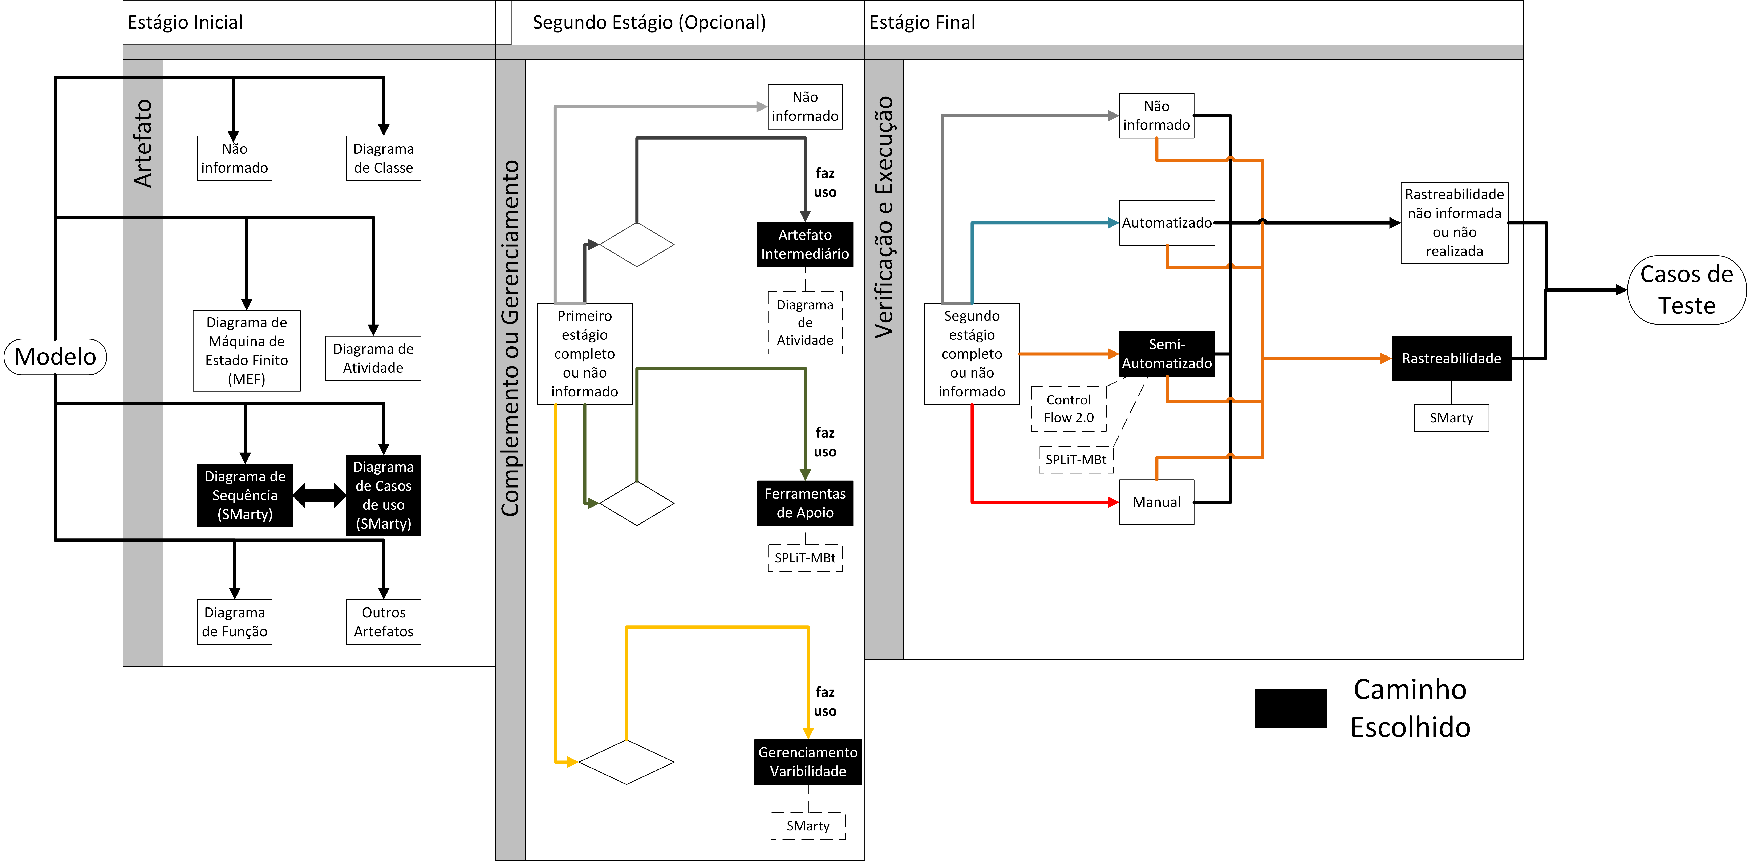
\includegraphics[scale=0.80]{roadmapcaminho2.pdf}
		\caption{Processo de geração de sequência de teste com \textit{SMartyTesting} (instância da \ref{fig:roadmap} )}
		\label{fig:roadmapcaminho}
	\end{figure}
\end{landscape}


\begin{figure}[h!]
	\centering
	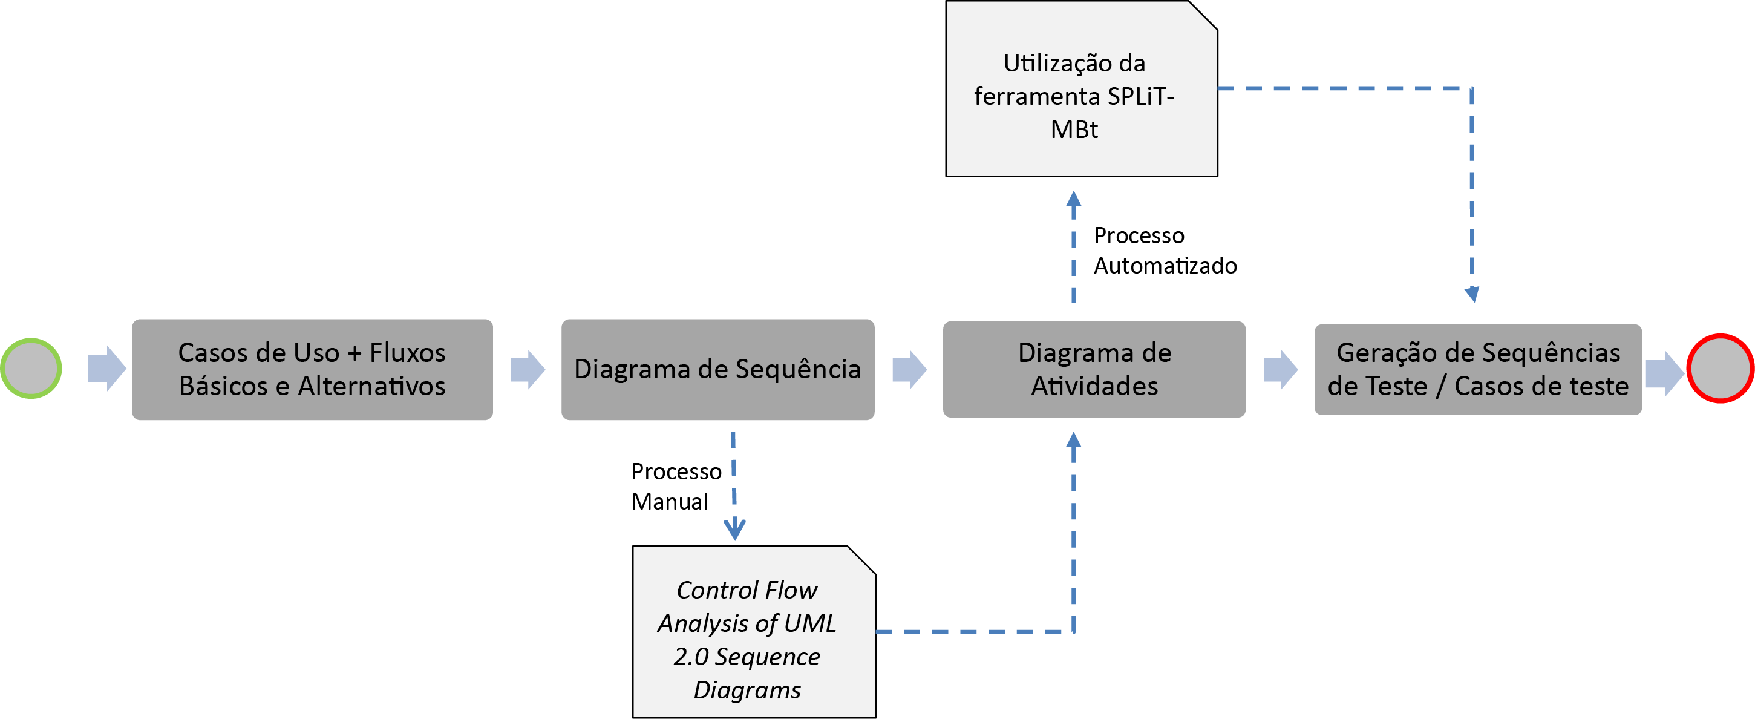
\includegraphics[scale=0.50]{ciclo_pesquisafinal.pdf}
	\caption{Passos para a geração de sequências de teste usando \textit{SMartyTesting}}
	\label{fig:ciclopesquisafinal}
\end{figure}


\subsection{Conversão de Diagramas de Sequência para Diagramas de Atividades}
\label{cap3subsec:conversaosequencia}


A conversão de diagramas de sequência para diagramas de atividades foi uma opção restritiva pelo fato de a ferramenta SPLiT-MBt ter como entrada diagramas de atividades. Embora também seja um diagrama de comunicação, o diagrama de atividades demonstra mais o fluxo de controle de uma atividade para outra, assim como a concorrência das atividades. Pode-se dizer que, enquanto o diagrama de sequência está mais próximo de métodos e do código-fonte, o diagrama de atividades está mais próximo dos casos de uso em termos de abstração.

Os dois diagramas são equivalentes quando se trata de elementos de representação, um exemplo é que em um diagrama de sequência, uma condicional de decisão pode ser representada por um diagrama de atividades, assim como quando um método, em um diagrama de sequência envia uma mensagem concorrente, criando uma bifurcação (\textit{fork}). 

Baseado no estudo de \citet{garousi2005control}, outro fator para a utilização de conversão de sequência para atividade é que não se corre o risco de perder propriedades no mapeamento, mantendo as características de variabilidades que foram estendidas no diagrama de sequência. Porém, é necessária uma validação desse mapeamento, o que foi feito por \citet{swain2010test}, sendo portanto, uma oportunidade para validação também com \textit{SMartyTesting}.

Por esses fatores é que se optou pela conversão de diagramas de sequência para atividades, aproveitando a validação da abordagem em uma ferramenta já desenvolvida SPLiT-MBt, que tem suporte à variabilidade, enquadrando-se no escopo deste trabalho.

A proposta de \citet{garousi2005control} consiste de uma metodologia de análise de fluxo de controle baseada em diagramas de sequência (DS) da UML 2.0. Essa técnica pode ser usada durante o ciclo de desenvolvimento e em outras abordagens de teste que façam compreensão e execução de modelos. Entre muitas aplicações, essa técnica pode ser usada em sistemas baseados em DS. 

Com base nos diagramas de atividades bem definidos, a proposta \textit{Control Flow Analysis of UML 2.0 Sequence Diagrams} (CCFG) \cite{garousi2005control} apresenta um metamodelo do diagrama de atividades estendido (\ref{fig:mapeamento2}), para apoiar a análise de fluxo de controle dos diagramas de sequência. Assim, pode-se definir um mapeamento baseado em \textit{Object Constraint Language} (OCL) \cite{warmer2003object} que é uma linguagem declarativa para descrever as regras que se aplicam aos modelos UML.

\begin{figure}[h!]
	\centering
	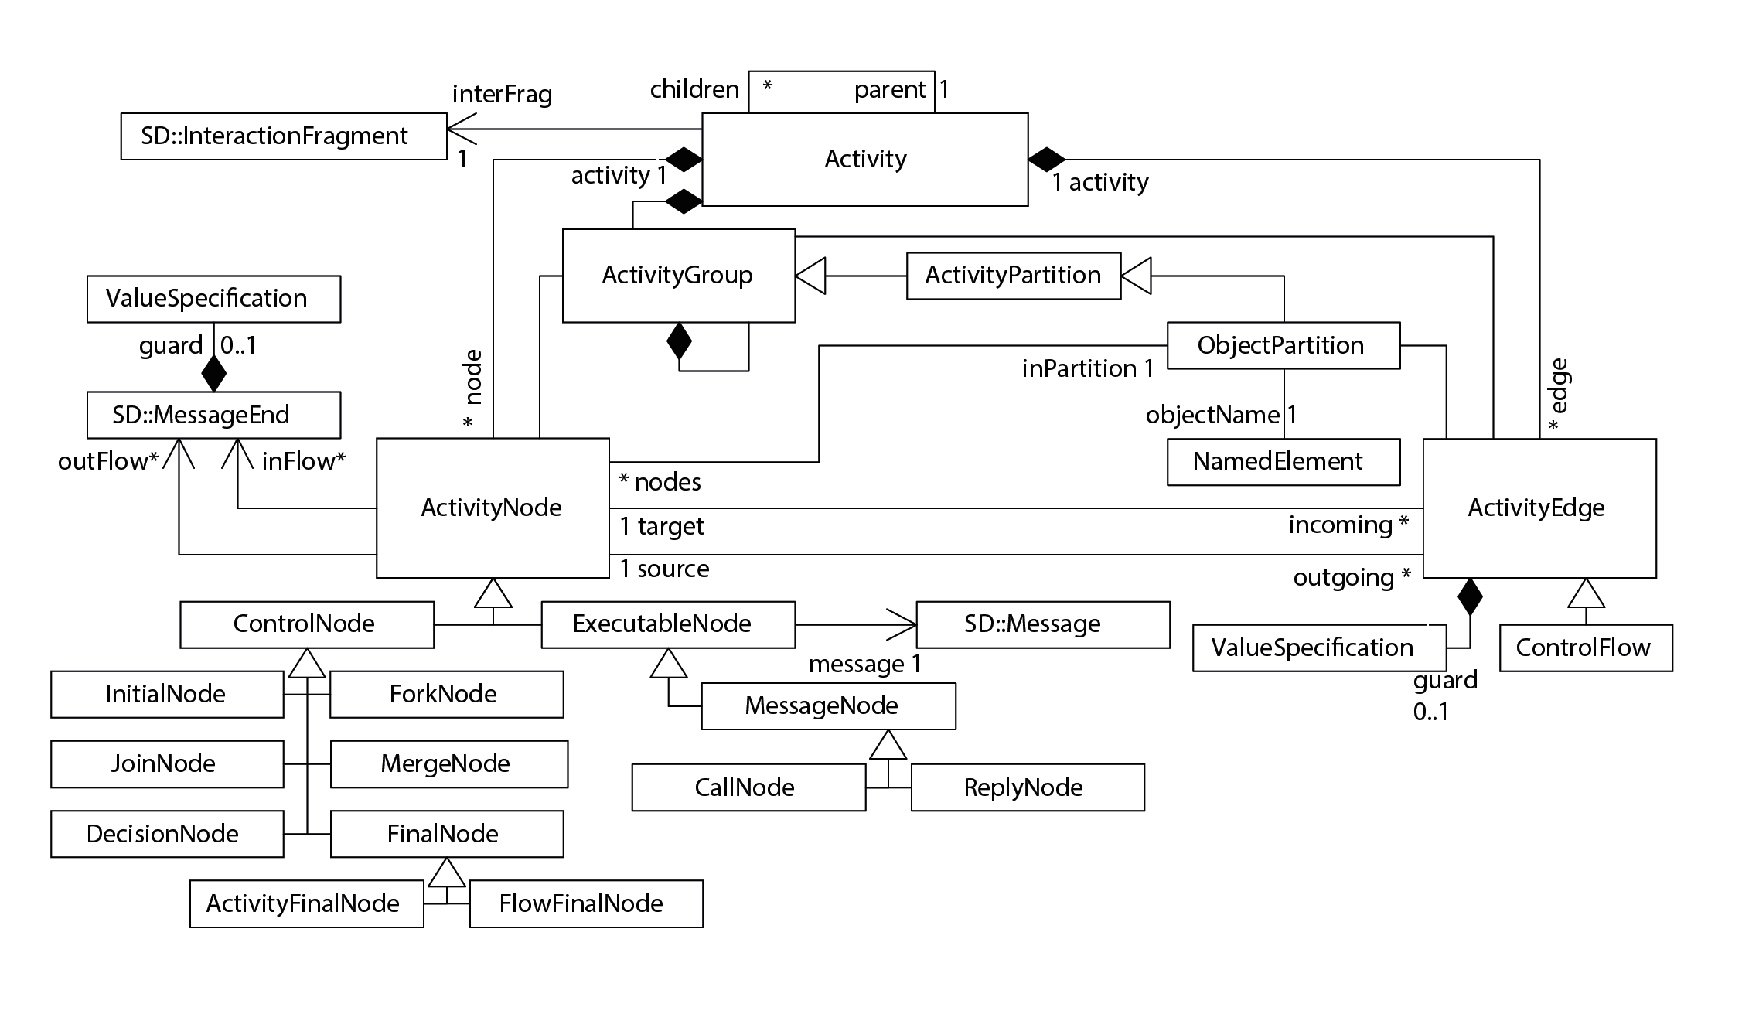
\includegraphics[scale=0.50]{atividade_metamodelo.pdf}
	\caption{Control Flow Analysis of UML 2.0 Sequence Diagrams metamodel (Diagramas de Atividades estendido) \cite{garousi2005control}}
	\label{fig:mapeamento2}
\end{figure}

A aplicação de OCL é realizada formalmente e verificável com regras de consistência entre um DS e um CCFG (diagramas de atividades estendido), em que CCFG possui todas as classes e associações necessárias, assim como suporte aos caminhos de fluxo de controle simultâneos (concorrência), que são uma generalização do conceito convencional de caminho de fluxo de controle \cite{garousi2005control}. 

O mapeamento consiste da utilização de um metamodelo DS (\ref{fig:mapeamento3}) e um conjunto de regras que deve ser utilizado na conversão, em que o metamodelo CCFG (\ref{fig:mapeamento2}) é considerado como validador.

\begin{figure}[h!]
	\centering
	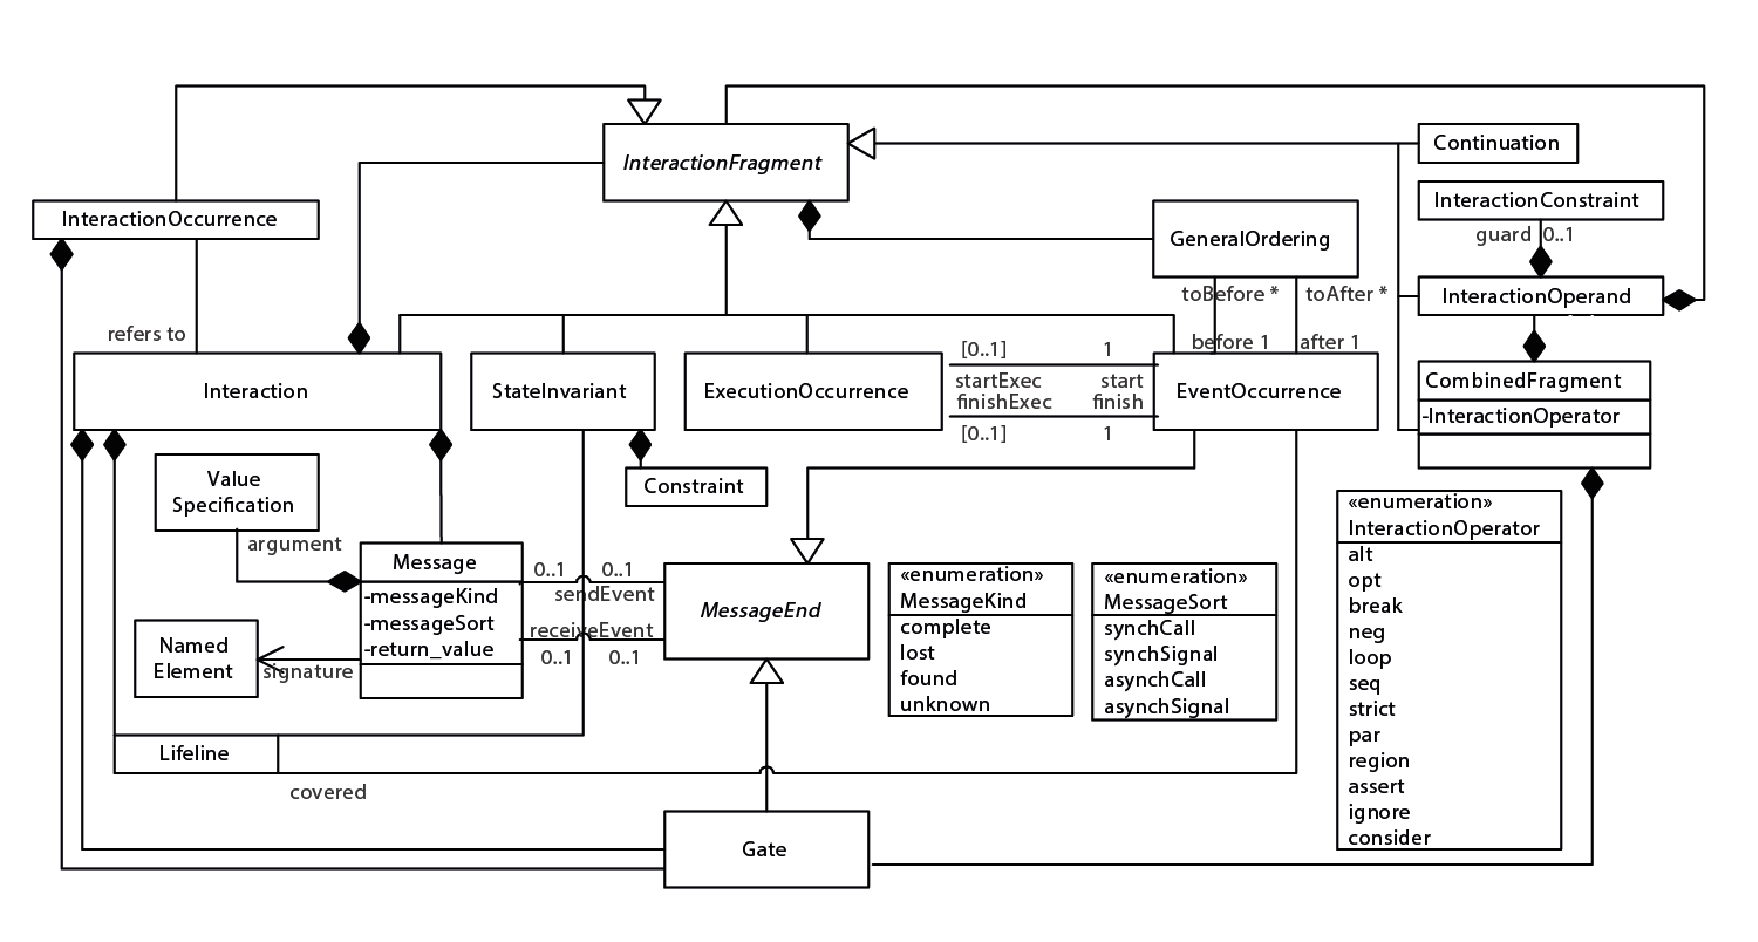
\includegraphics[scale=0.50]{sequencia_metamodelo.pdf}
	\caption{Metamodelo de diagramas de sequência UML \cite{garousi2005control}}
	\label{fig:mapeamento3}
\end{figure}

Como exemplo, tem-se diagramas de sequência (\ref{fig:mapeamento1}) que aparenta mensagens assíncronas. Para realizar o mapeamento para atividades (CCFG) foi utilizado um conjunto de regras criadas a partir dos metamodelos \cite{garousi2005control}. As regras são apresentadas na \ref{tab:regrasmapeamento}. Com isso, o processo de mapeamento deu origem ao diagrama de atividades apresentado na \ref{fig:mapeamento4}.   

\begin{figure}[h!]
	\centering
	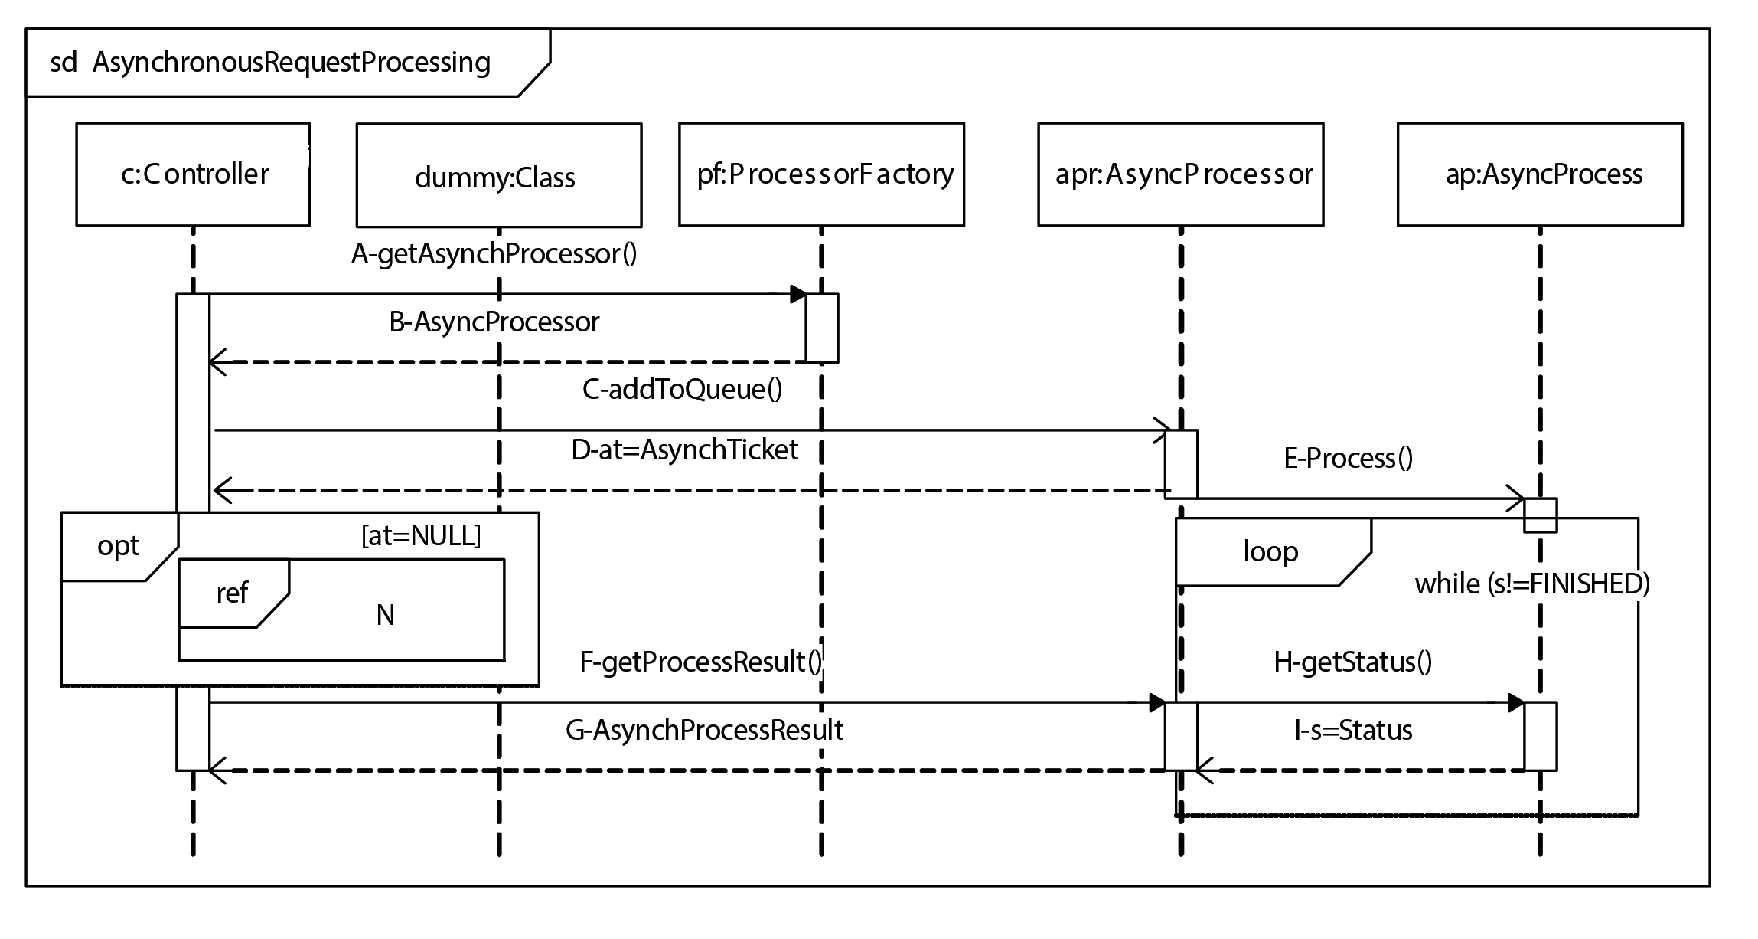
\includegraphics[scale=0.50]{diag_sequencia.pdf}
	\caption{Um diagrama de sequência com mensagens assíncronas \cite{garousi2005control}}
	\label{fig:mapeamento1}
\end{figure}


\begin{table}[h!]
	\centering
	\caption{Regras utilizadas para a conversão de DS para DA \cite{garousi2005control}}
	\label{tab:regrasmapeamento}
	\begin{tabular}{c|l|l}
		\hline
		\textbf{N°} & \multicolumn{1}{c|}{\textbf{Recurso do DS}} & \multicolumn{1}{c}{\textbf{Recurso do CCFG (Atividades)}} \\ \hline
		1 & Interaction & Activity \\ \hline
		2 & First message end & \begin{tabular}[c]{@{}l@{}}Flow between InitialNode\\ and first control node\end{tabular} \\ \hline
		3 & SynchCall/SynchSignal & CallNode \\ \hline
		4 & AsynchCall or AsynchSignal & \begin{tabular}[c]{@{}l@{}}(CallNode+ForkNode) or\\ ReplyNode\end{tabular} \\ \hline
		5 & \begin{tabular}[c]{@{}l@{}}Message SendEvent and\\ ReceiveEvent\end{tabular} & ControlFlow \\ \hline
		6 & Lifeline & ObjectPartition \\ \hline
		7 & par CombinedFragment & ForkNode \\ \hline
		8 & loop CombinedFragment & DecisionNode \\ \hline
		9 & alt/opt CombinedFragment & DecisionNode \\ \hline
		10 & break CombinedFragment & ActivityEdge \\ \hline
		11 & Last message ends & \begin{tabular}[c]{@{}l@{}}Flow between end control\\ nodes and FinalNode\end{tabular} \\ \hline
		12 & InteractionOccurrence & Control Flow across CCFGs \\ \hline
		13 & Polymorphic message & DecisionNode \\ \hline
		14 & Nested InteractionFragmen & Nested CCFGs \\ \hline
	\end{tabular}
\end{table}


\begin{figure}[H]
	\centering
	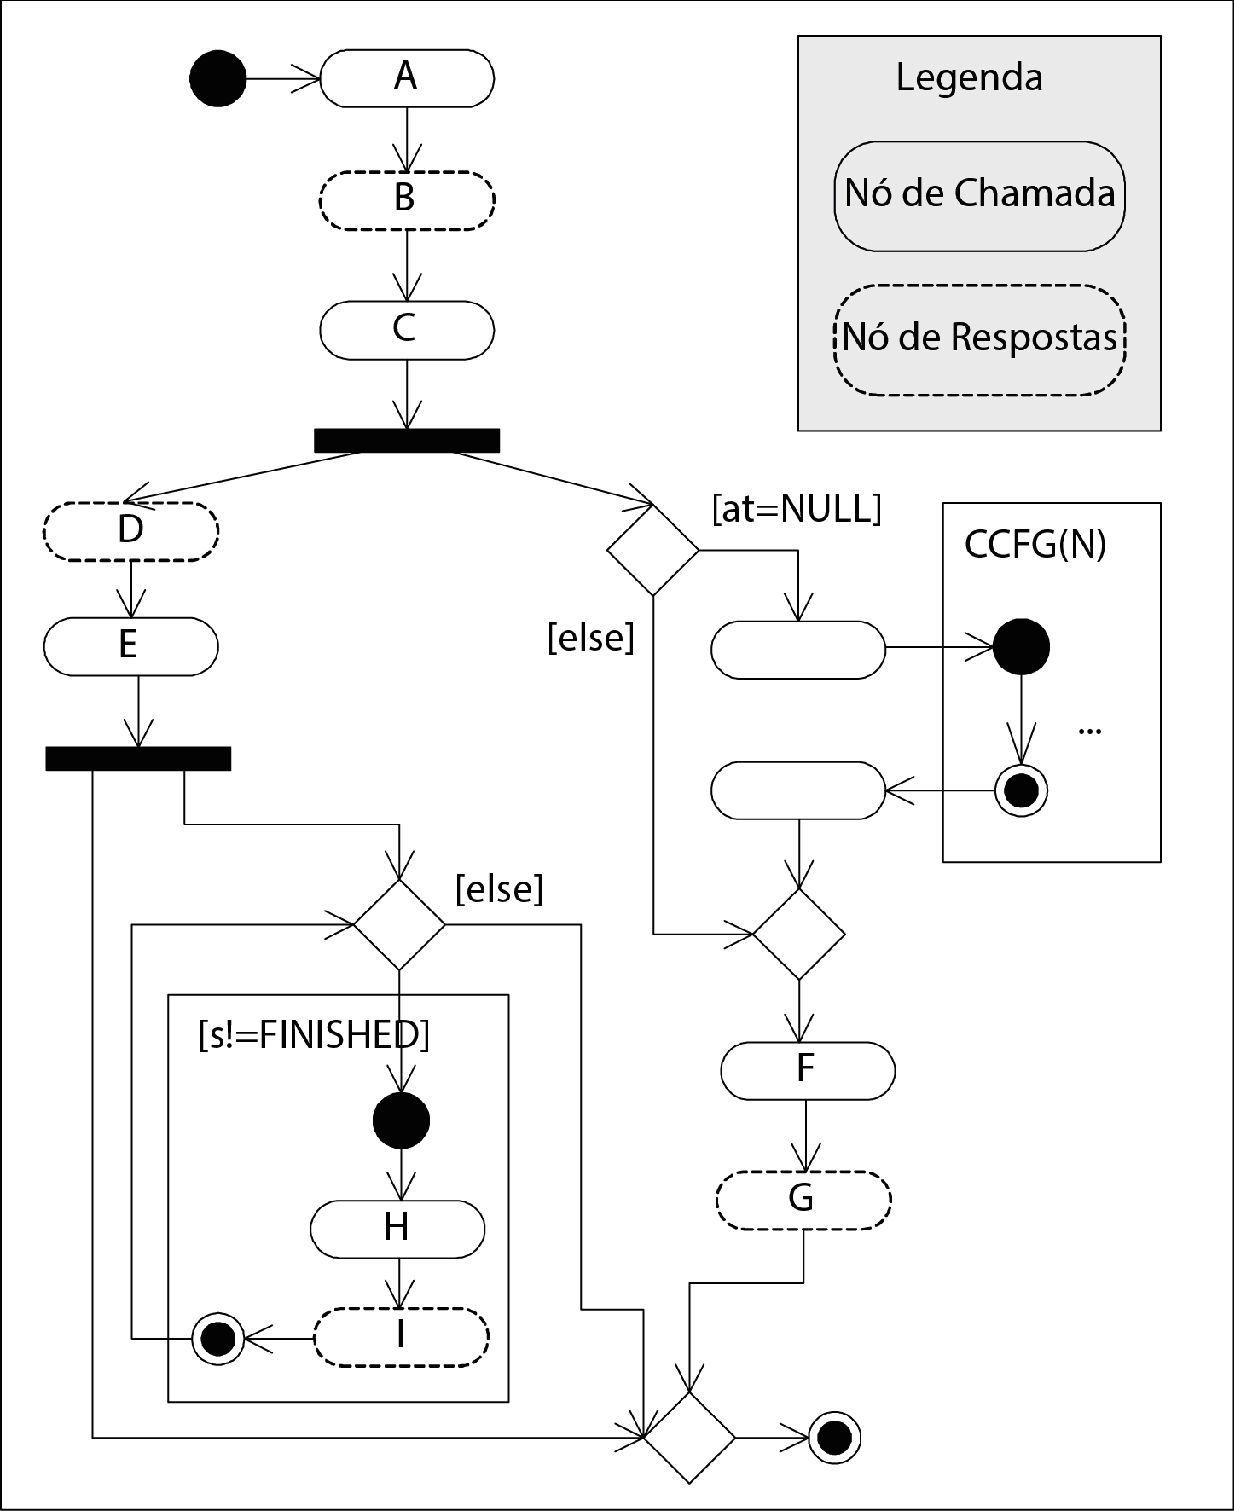
\includegraphics[scale=0.40]{sequencia_result_map.pdf}
	\caption{Resultado do mapeamento do DS da \ref{fig:mapeamento1}. Traduzido de \citet{garousi2005control}}
	\label{fig:mapeamento4}
\end{figure}

Para a validação da abordagem \textit{SMartyTesting} foi realizada a conversão manual dos DSs para DAs utilizando a ferramenta \textit{Astah professional 6}\footnote[1]{Disponível em: http://astah.net/download - Acessado em 20/10/2019}. Ao final da criação dos diagramas, os mesmos foram exportados com extensão XML, para serem utilizados na segunda etapa por SPLiT-MBt.

  
\subsection{Ferramenta Utilizada}
\label{cap3sec:ferramenta_utilizada_split}


SPLiT-MBt faz o uso do método de geração HSI. A razão para a escolha desse método se deve ao fato de ser um dos métodos menos restritivos em relação às propriedades que as MEFs devem ter. Por exemplo, o HSI é capaz de interpretar MEFs completas e parciais \cite{petrenko1994nondeterministic}. 

Além disso, o método HSI permite cobertura total de falhas existentes e gera sequências de teste menores que outros métodos, o que contribui para a otimização do processo de teste. Esses fatores são muito relevantes no contexto da LPS, porque quanto maior o número de \textit{features} de uma LPS, maior é o número de casos de teste necessários para testar produtos da LPS \cite{engstrom2011software}.

Como houve necessidade de se estender a abordagem por causa da variabilidade, para gerar sequências de teste a partir de uma versão estendida do HSI, foi necessário aplicar o método considerando as informações de variabilidade presentes no MEF. 

A SPLiT-MBt aceita, inicialmente, um arquivo de entrada em formato \textit{eXtensible Markup Language} (XML), faz a leitura do arquivo e valida todos os requisitos de entrada do artefato. Caso esteja correto, monta-se a estrutura e, assim que o usuário clica na opção de geração, SPLiT-MBt converte o DA em MEF em tempo de execução e realiza o processo de geração de sequências de teste.


\section{Especificação da Abordagem \textit{SMartyTesting}}
\label{cap3sec:especificacao_smarty}
Nesta seção é apresentado cada passo da abordagem \textit{SMartyTesting}. Neste trabalho, parte-se do princípio de que a modelagem de casos de uso tenha dado origem aos diagramas de sequência.

\subsection{Etapa 1 - Mapeamento de Diagramas de Sequência para Diagramas de Atividades}
\label{cap3subsec:etapa1}

Nesta primeira etapa foi realizado o mapeamento dos diagramas de sequência (DS) para o de atividades estendido (DA). Para tanto, foi usada a LPS AGM. A etapa 1 é ilustrada na \ref{fig:SM_etapa1}. 

\begin{figure}[h!]
	\centering
	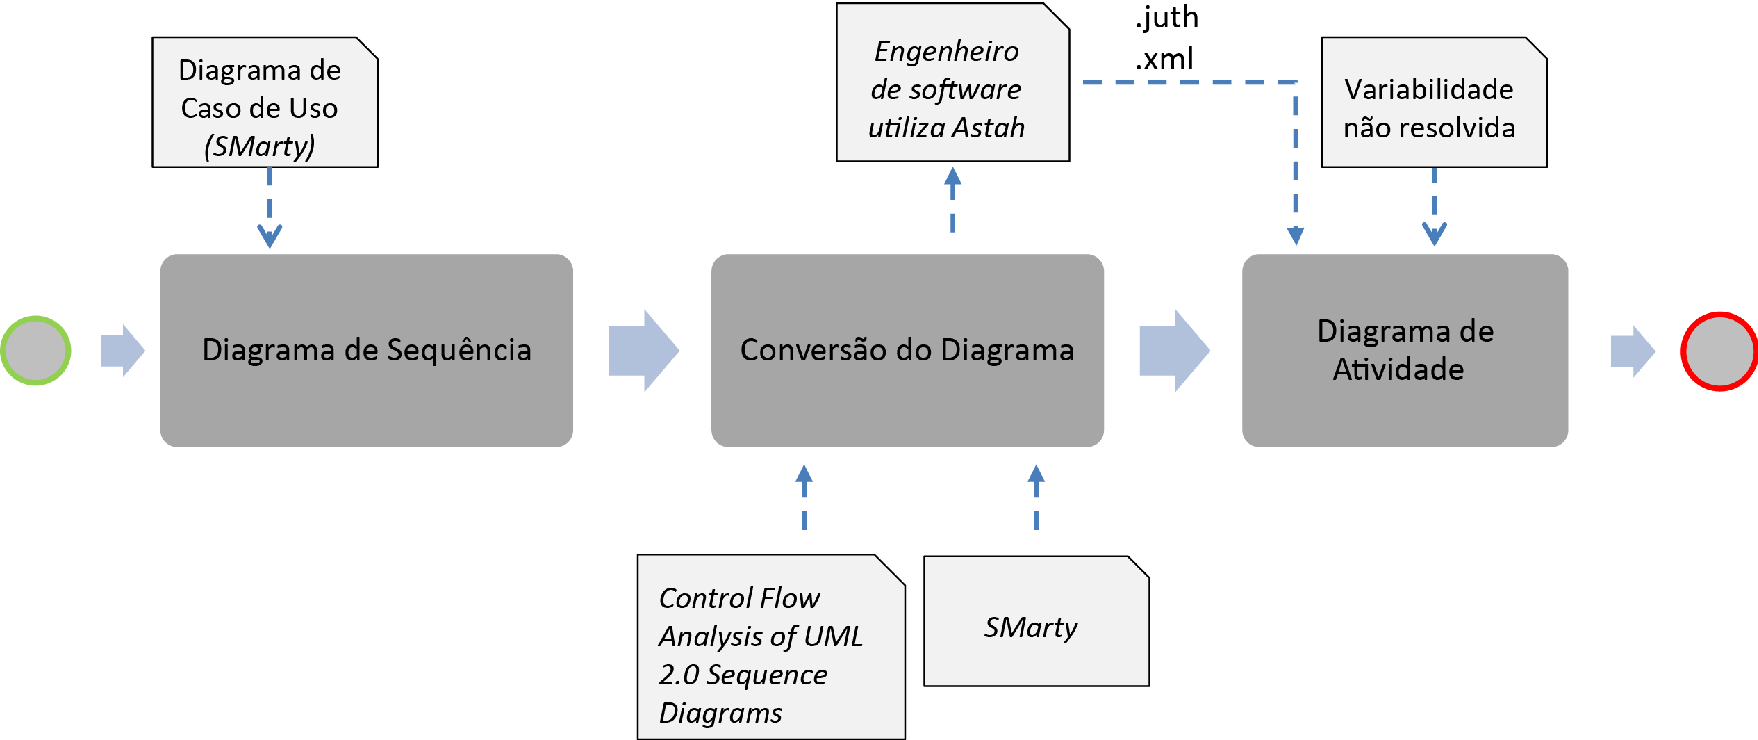
\includegraphics[scale=0.50]{etapa1_ds_to_da.pdf}
	\caption{Ciclo da etapa 1}
	\label{fig:SM_etapa1}
\end{figure}


O DS foi modelado considerando a abordagem \textit{SMarty} utilizando a ferramenta \textit{Cameo Enterprise Architecture} versão 19 \footnote{\url{https://www.nomagic.com/products/cameo-enterprise-architecture}}. Depois de modelado o diagrama de sequência e todas as suas propriedades (\ref{fig:exemploDS}), o engenheiro de software deverá construir um novo diagrama de atividades, porém levando em consideração as regras da \ref{tab:regrasmapeamento} e as propriedades do diagrama de sequência criado.


\begin{figure}[h!]
	\centering
	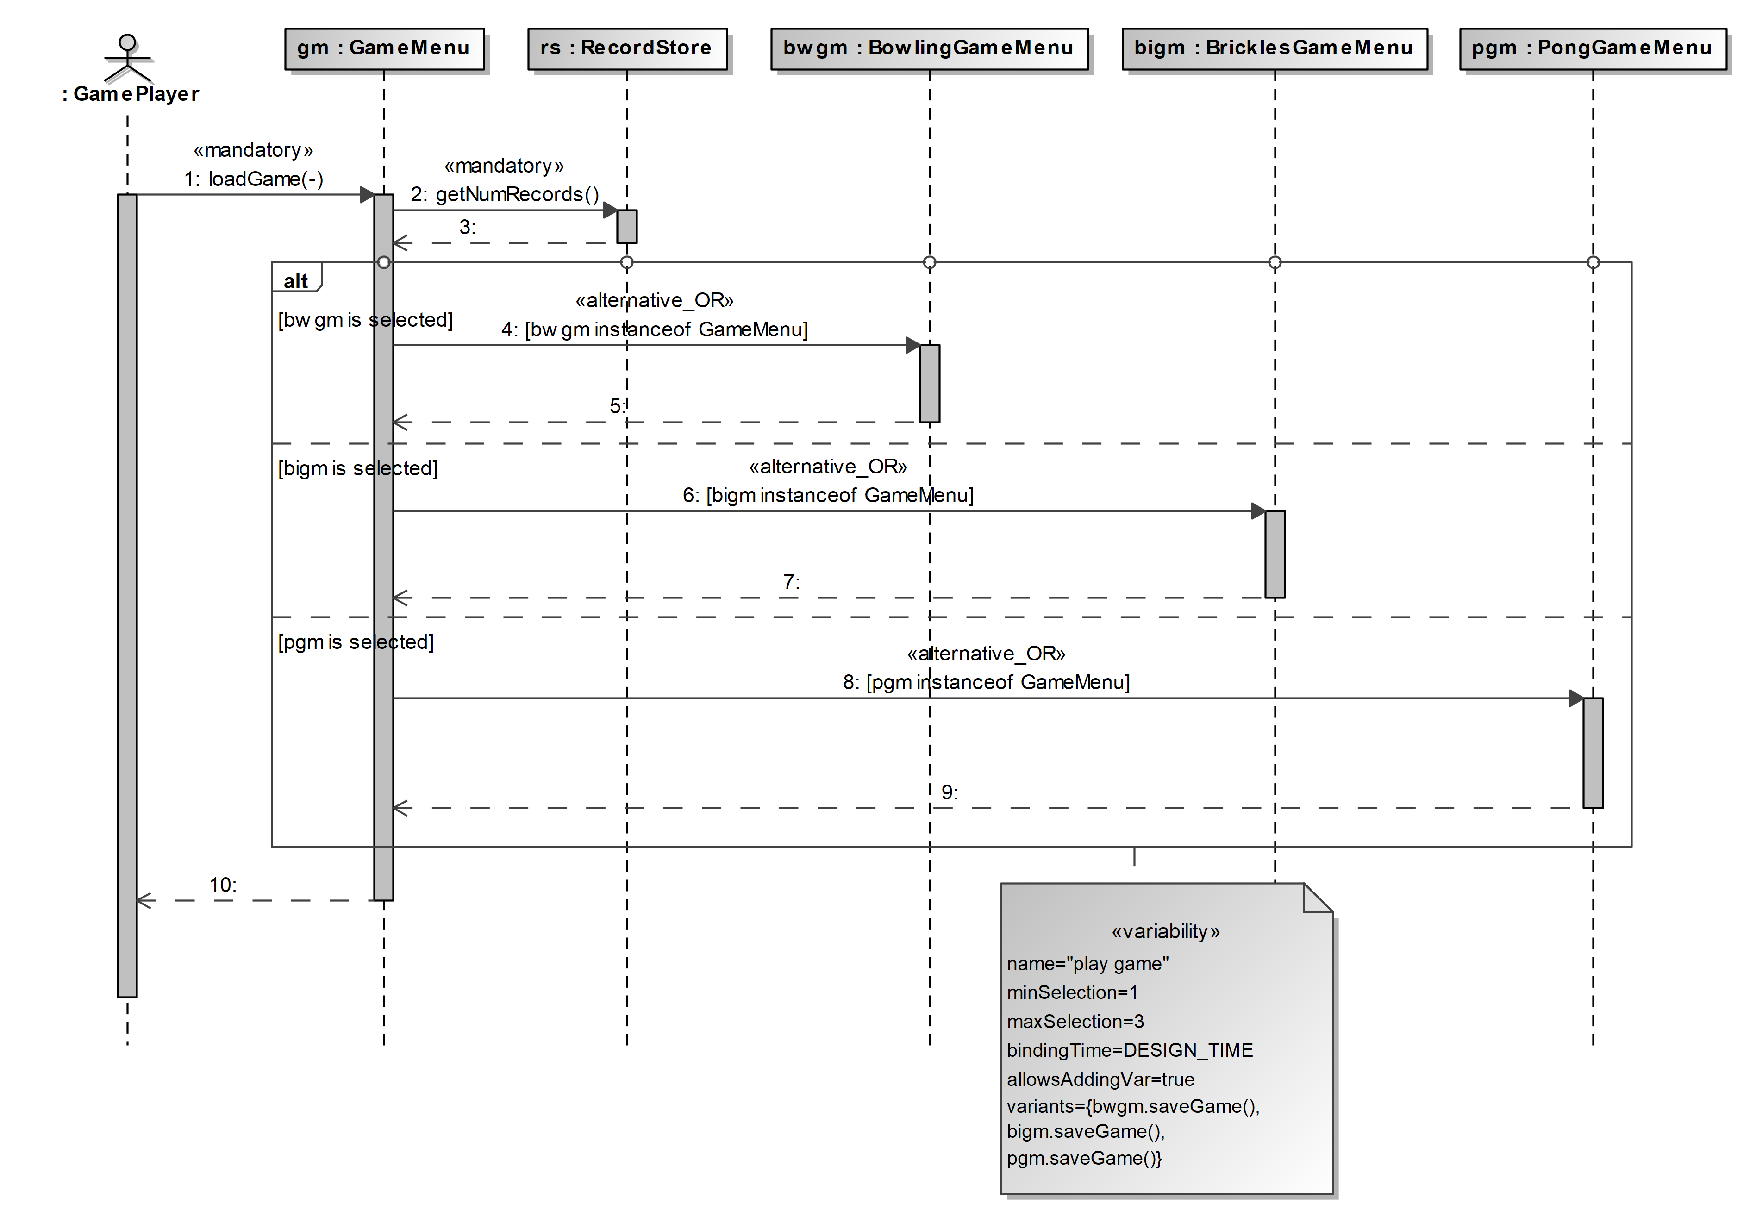
\includegraphics[scale=0.47]{exemploDS.pdf}
	\caption{Diagramas de sequência ilustrando o caso de uso \textit{game menu} da AGM}
	\label{fig:exemploDS}
\end{figure}

Neste trabalho utilizou-se outra ferramenta (IDE) de modelagem para a criação do modelo convertido de DS para DA, a ferramenta utilizada foi a \textit{Astah} versão 6. Optou-se por essa versão a fim de demonstrar que mesmo com IDEs diferentes para modelagem, pode-se chegar ao mesmo resultado esperado.

A criação do DA deve levar em consideração o uso das regras de mapeamento contidas na \ref{tab:regrasmapeamento}, as propriedades de variabilidade são mantidas sem a resolução, a fim de serem transportadas às sequências de teste para serem reutilizadas. A \ref{fig:exemploDA} apresenta o resultado da conversão do DS da \ref{fig:exemploDS}.

Na execução da construção do DA deve-se levar em consideração os requisitos necessários que serão utilizados na Etapa 2. O arquivo do artefato modelado deve ser exportado da ferramenta em formato XML, que é o formato de entrada suportado por SPLiT-MBt.

\begin{figure}[H]
	\centering
	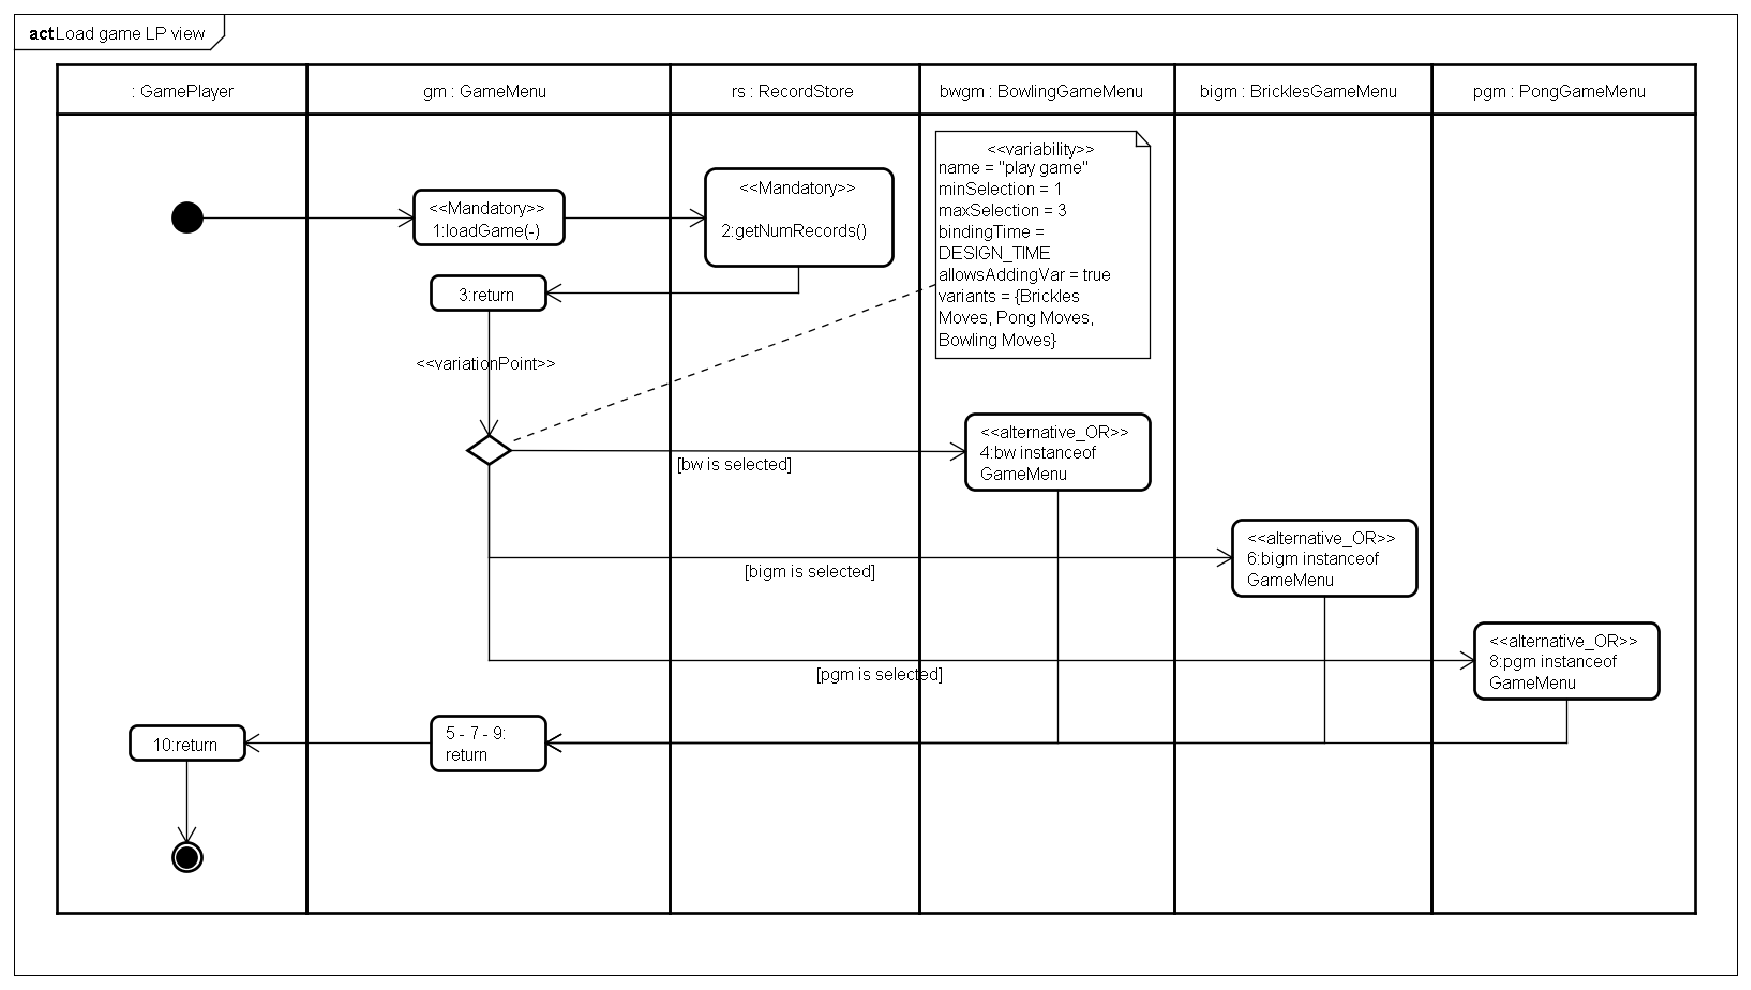
\includegraphics[scale=0.55]{exemploDA.pdf}
	\caption{Diagramas de atividades resultante do mapeamento do DS da \ref{fig:exemploDS}}
	\label{fig:exemploDA}
\end{figure}

Para a utilização do arquivo do artefato de DA, antes da exportação pela IDE, devem ser levadas em consideração algumas características. Uma delas é a parametrização das transições do DA, necessárias para utilização na ferramenta SPLiT-MBt. Deve ser levado em consideração também o estereótipo da atividade que está sendo modelada fazendo uso de \textit{SMarty}.

Esses parâmetros são informações referentes às transições no DA. Assim, tem-se a transição da atividade, na que está contida a \textit{tag} identificando qual é a ação (\textit{TDaction}) e o resultado esperado (\textit{TDexpectedResult}) e, por fim, os valores (\textit{Values}) que são adicionados conforme as especificações do DA. A \ref{fig:exemploTAG} apresenta uma visão dessa configuração necessária. 

\begin{figure}[H]
	%\centering
	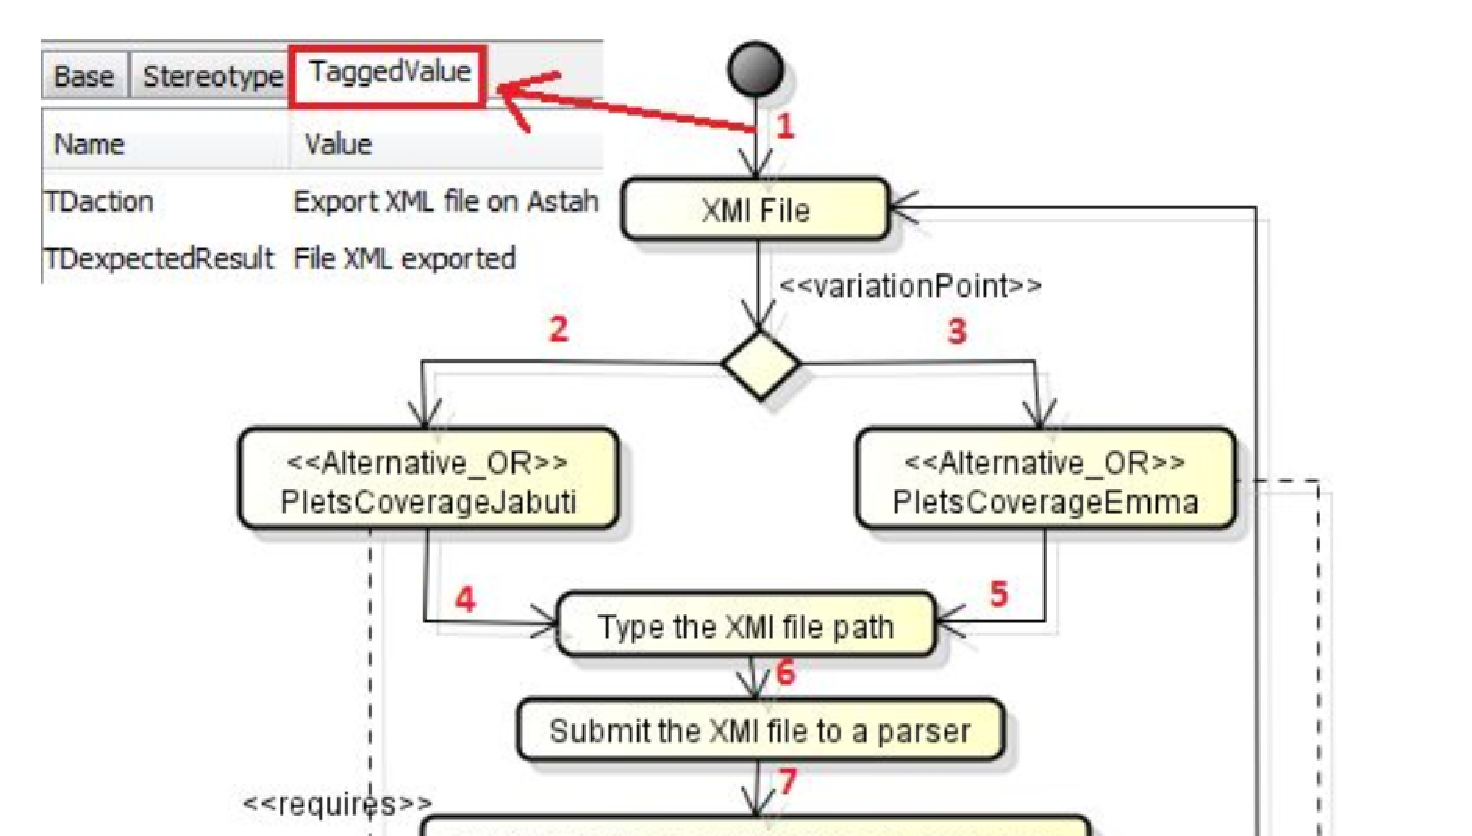
\includegraphics[scale=0.50]{exemploTAG.pdf}
	\caption{Exemplificação da parametrização dos \textit{controlflows} de um diagrama de atividades usando SPLiT-MBt \cite{costa2016split}}
	\label{fig:exemploTAG}
\end{figure}

Seguindo essa parametrização necessária, a \ref{tab:valores_tag} apresenta todos os parâmetros das transições do DA resultante do mapeamento.


%\begin{landscape}
	\begin{table}[H]
	    \footnotesize
		\caption{Valores dos atributos de parametrização do DA para utilização em SPLiT-MBt}
		\label{tab:valores_tag}
		\begin{tabular}{l|l|l}
			\hline
			\textbf{Transição das Atividades} & \textbf{Tags} & \textbf{Valores} \\ \hline
			\begin{tabular}[c]{@{}l@{}}1- Estágio Inicial \\ para LoadGame\end{tabular} & \begin{tabular}[c]{@{}l@{}}TDaction\\ TDexpectedResult\end{tabular} & \begin{tabular}[c]{@{}l@{}}- Game Player faz o carregamento do jogo\\ - Jogo carrega\end{tabular} \\ \hline
			\begin{tabular}[c]{@{}l@{}}2- LoadGame \\ para getNumRecords\end{tabular} & \begin{tabular}[c]{@{}l@{}}TDaction\\ TDexpectedResult\end{tabular} & \begin{tabular}[c]{@{}l@{}}- Game menu faz acesso ao dados de pontuação\\ - Consegue acesso ao dados de pontuação\end{tabular} \\ \hline
			\begin{tabular}[c]{@{}l@{}}3- getNumRecords \\ para return\end{tabular} & \begin{tabular}[c]{@{}l@{}}TDaction\\ TDexpectedResult\end{tabular} & \begin{tabular}[c]{@{}l@{}}- recordStore retorna os dados\\ - Dados de pontuação são retornados\end{tabular} \\ \hline
			\begin{tabular}[c]{@{}l@{}}4- Decision node para \\ bw instanceof GameMenu\end{tabular} & \begin{tabular}[c]{@{}l@{}}TDaction\\ TDexpectedResult\end{tabular} & \begin{tabular}[c]{@{}l@{}}- Opção bw é selecionada\\ - Acesso aos recurso da opção bw\end{tabular} \\ \hline
			5- return & \begin{tabular}[c]{@{}l@{}}TDaction\\ TDexpectedResult\end{tabular} & \begin{tabular}[c]{@{}l@{}}- Retorno da opção bw\\ - Retorne ao menu de opções\end{tabular} \\ \hline
			\begin{tabular}[c]{@{}l@{}}6- Decision node para \\ bigm instanceof GameMenu\end{tabular} & \begin{tabular}[c]{@{}l@{}}TDaction\\ TDexpectedResult\end{tabular} & \begin{tabular}[c]{@{}l@{}}- Opção bigm é selecionada\\ - Acesso aos recurso da opção bigm\end{tabular} \\ \hline
			7- return & \begin{tabular}[c]{@{}l@{}}TDaction\\ TDexpectedResult\end{tabular} & \begin{tabular}[c]{@{}l@{}}- Retorno da opção bigm\\ - Retorne ao menu de opções\end{tabular} \\ \hline
			\begin{tabular}[c]{@{}l@{}}8- Decision node para \\ pgm instanceof GameMenu\end{tabular} & \begin{tabular}[c]{@{}l@{}}TDaction\\ TDexpectedResult\end{tabular} & \begin{tabular}[c]{@{}l@{}}- Opção pgm é selecionada\\ - Acesso aos recurso da opção pgm\end{tabular} \\ \hline
			9- return & \begin{tabular}[c]{@{}l@{}}TDaction\\ TDexpectedResult\end{tabular} & \begin{tabular}[c]{@{}l@{}}- Retorno da opção pgm\\ - Retorne ao menu de opções\end{tabular} \\ \hline
			10- return & \begin{tabular}[c]{@{}l@{}}TDaction\\ TDexpectedResult\end{tabular} & \begin{tabular}[c]{@{}l@{}}- Retorno da informação ao Game Player\\ - Player recebe retorno da ação escolhida\end{tabular} \\ \hline
		\end{tabular}
	\end{table}
%\end{landscape}


\subsection{Etapa 2 - Geração de Sequências de Teste}
\label{cap3subsec:etapa2}

Na segunda etapa considera-se que o DS já tenha sido mapeado e convertido para DA, conforme o fluxo apresentado na \ref{fig:SM_etapa2}. Dado o mapeamento de conversão realizado faz-se a geração de sequências de casos de teste. 

\begin{figure}[H]
	\centering
	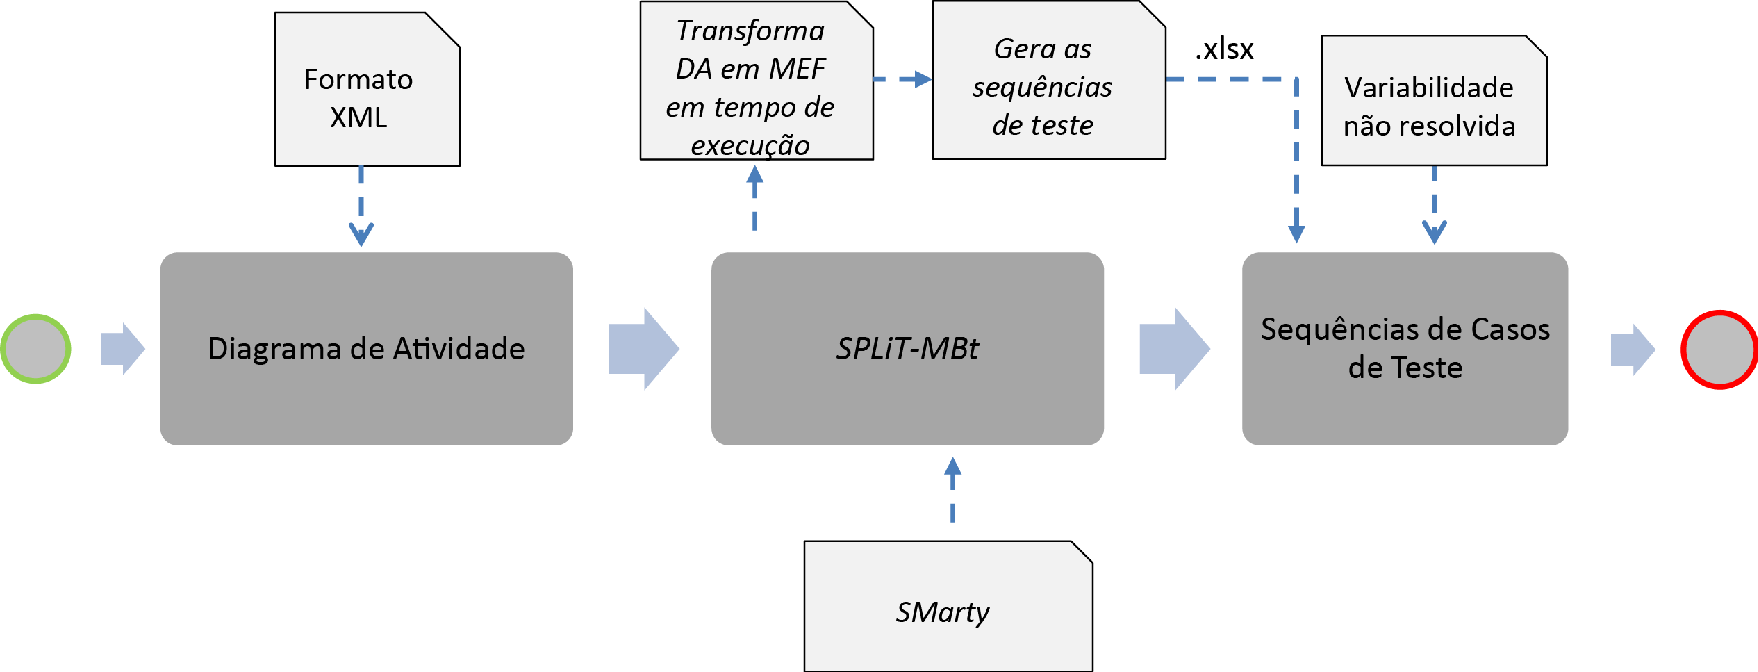
\includegraphics[scale=0.52]{etapa2_da_to_caso.pdf}
	\caption{Ciclo da etapa 2}
	\label{fig:SM_etapa2}
\end{figure}


De posse do arquivo XML gerado, inicia-se o carregamento do arquivo na ferramenta (\ref{fig:split_carregamento}). Após o arquivo ser carregado pela aplicação, faz-se a verificação da estrutura do arquivo XML (\ref{fig:split_validacao}).

\begin{figure}[h!]
	\centering
	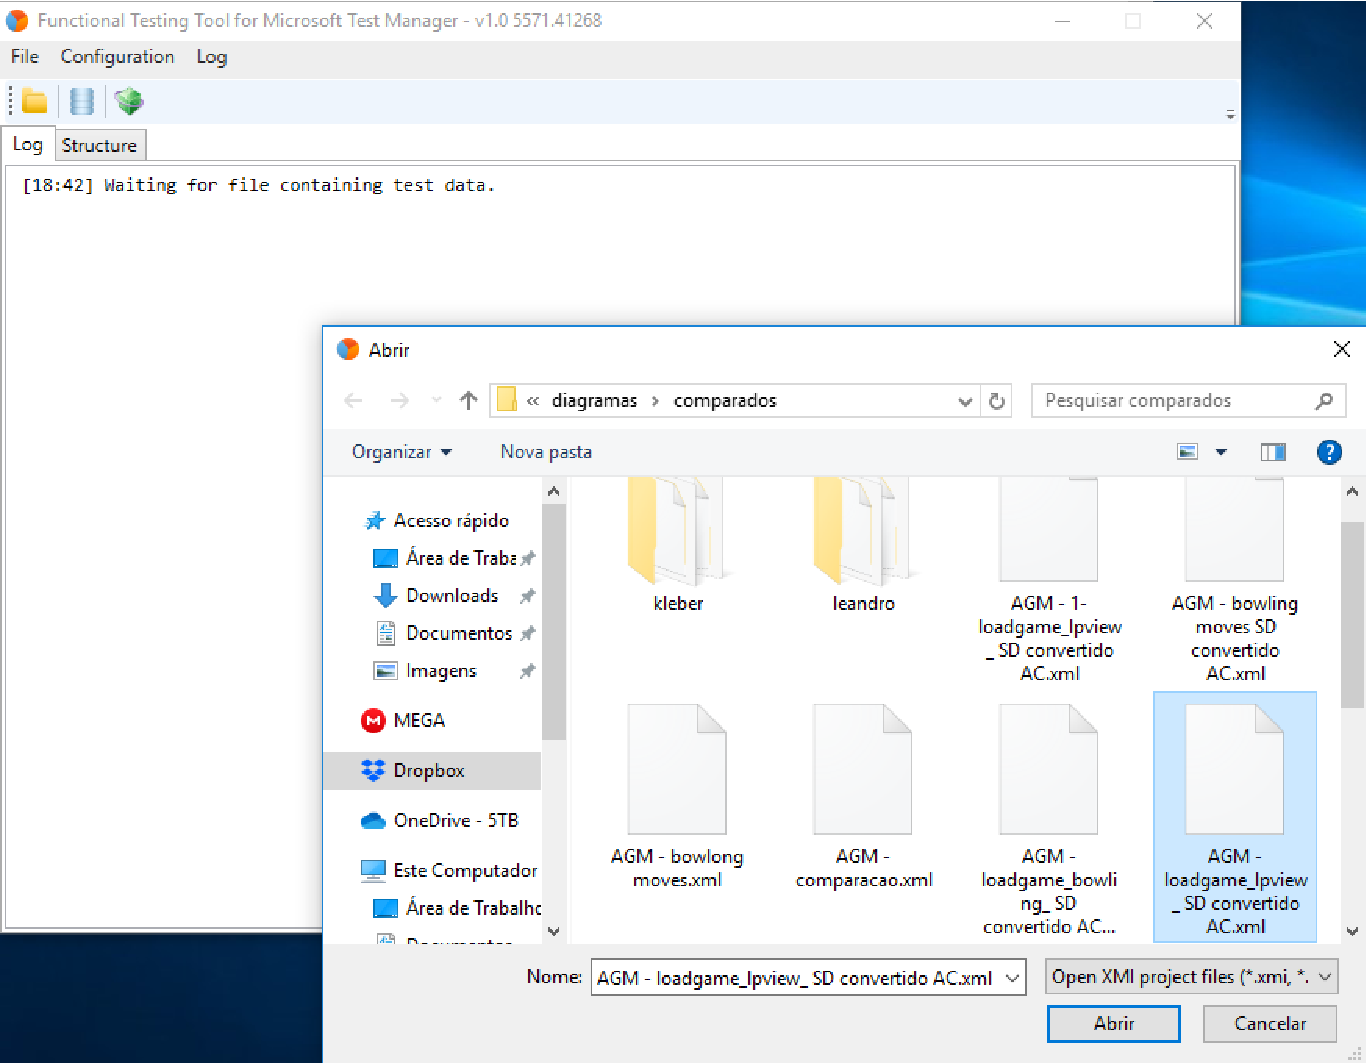
\includegraphics[scale=0.60]{splitcarregamento.pdf}
	\caption{Tela de carregamento de arquivo da ferramenta SPLiT-MBt}
	\label{fig:split_carregamento}
\end{figure}


\begin{figure}[h!]
	\centering
	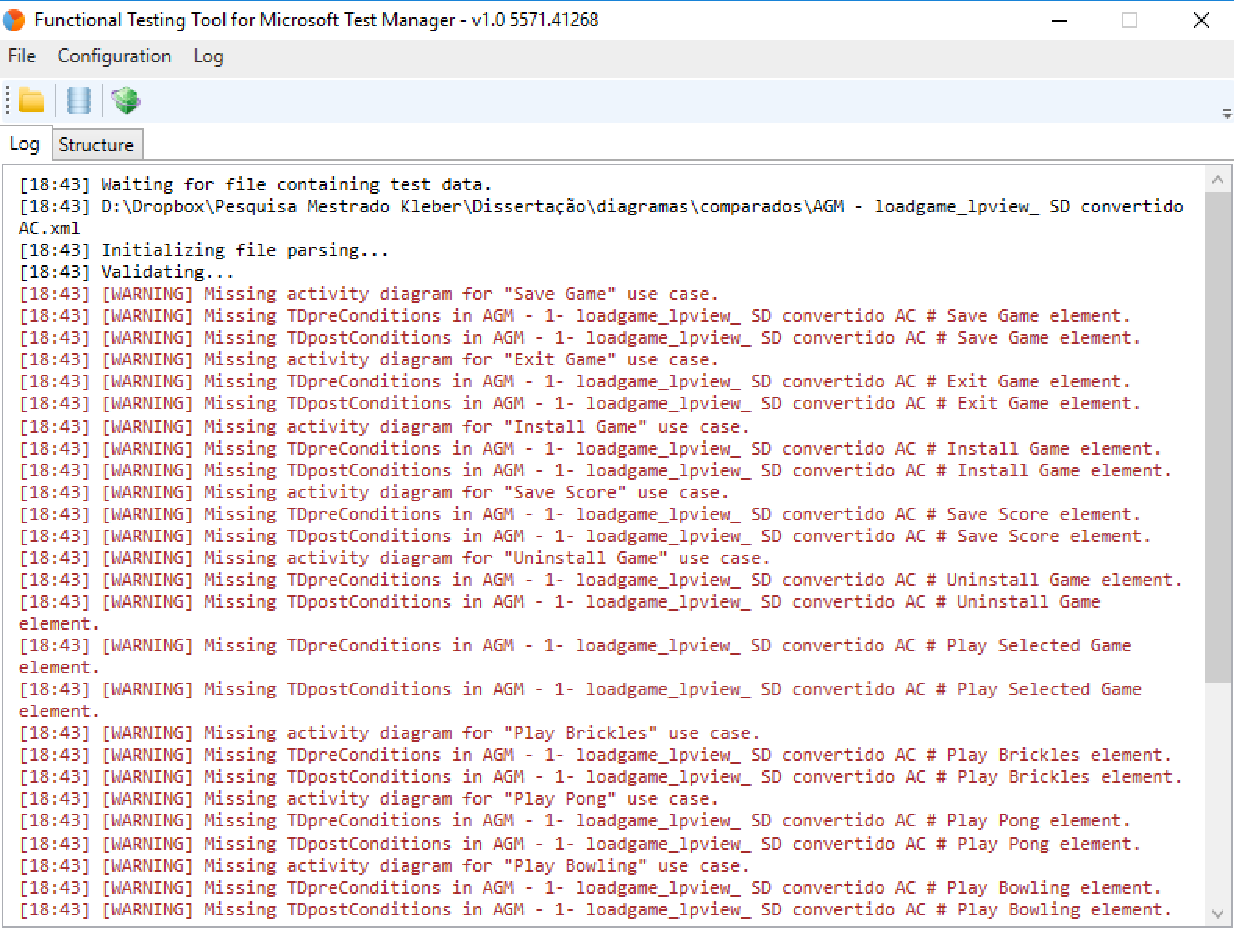
\includegraphics[scale=0.55]{splitvalidacao.pdf}
	\caption{Validação da estrutura do arquivo carregado pela SPLiT-MBt}
	\label{fig:split_validacao}
\end{figure}

Após a validação do arquivo que é carregado, pode ser observada a sua estrutura usando a própria ferramenta (\ref{fig:split_estrutura}), com isso pode-se realizar a geração de casos de teste e, quando não houver erros na geração, a mensagem de sucesso é apresentada (\ref{fig:split_gerado}).  

\begin{figure}[h!]
	\centering
	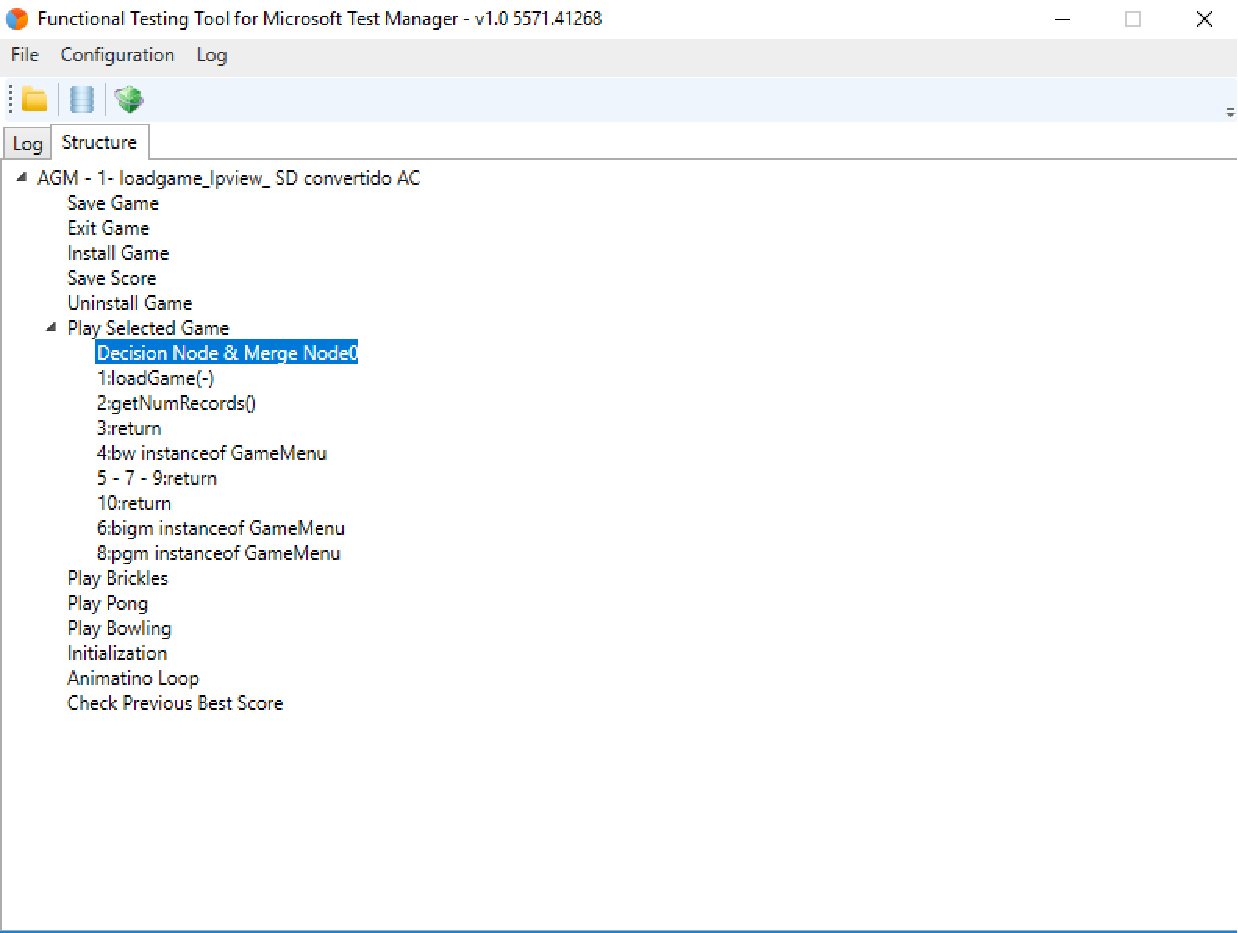
\includegraphics[scale=0.55]{splitestrutura.pdf}
	\caption{Apresentação da estrutura do arquivo XML}
	\label{fig:split_estrutura}
\end{figure}


No momento da geração a ferramenta faz a conversão do DA em MEFs estendidas para suportar variabilidade. Essa conversão é realizada em tempo de execução, assim, não há acesso a nenhum arquivo ou processo, tornando a execução um processo interno da ferramenta.

\begin{figure}[h!]
	\centering
	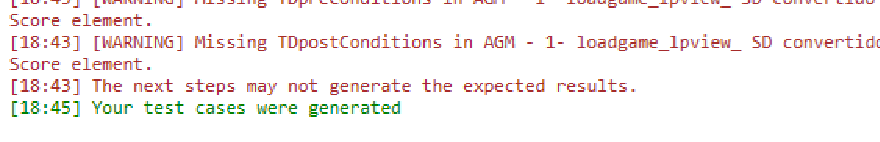
\includegraphics[scale=0.75]{splitgerado.pdf}
	\caption{Mensagem de sucesso na geração dos casos de teste}
	\label{fig:split_gerado}
\end{figure}

Após a geração, é possível exportar um arquivo XLSx, que é umdos formatos de extensão aceitados pelo Excel, (\ref{fig:split_casodeteste}) que pode ser utilizado em ferramentas de teste que fazem uso de \textit{scripts}.

\begin{figure}[h!]
	\centering
	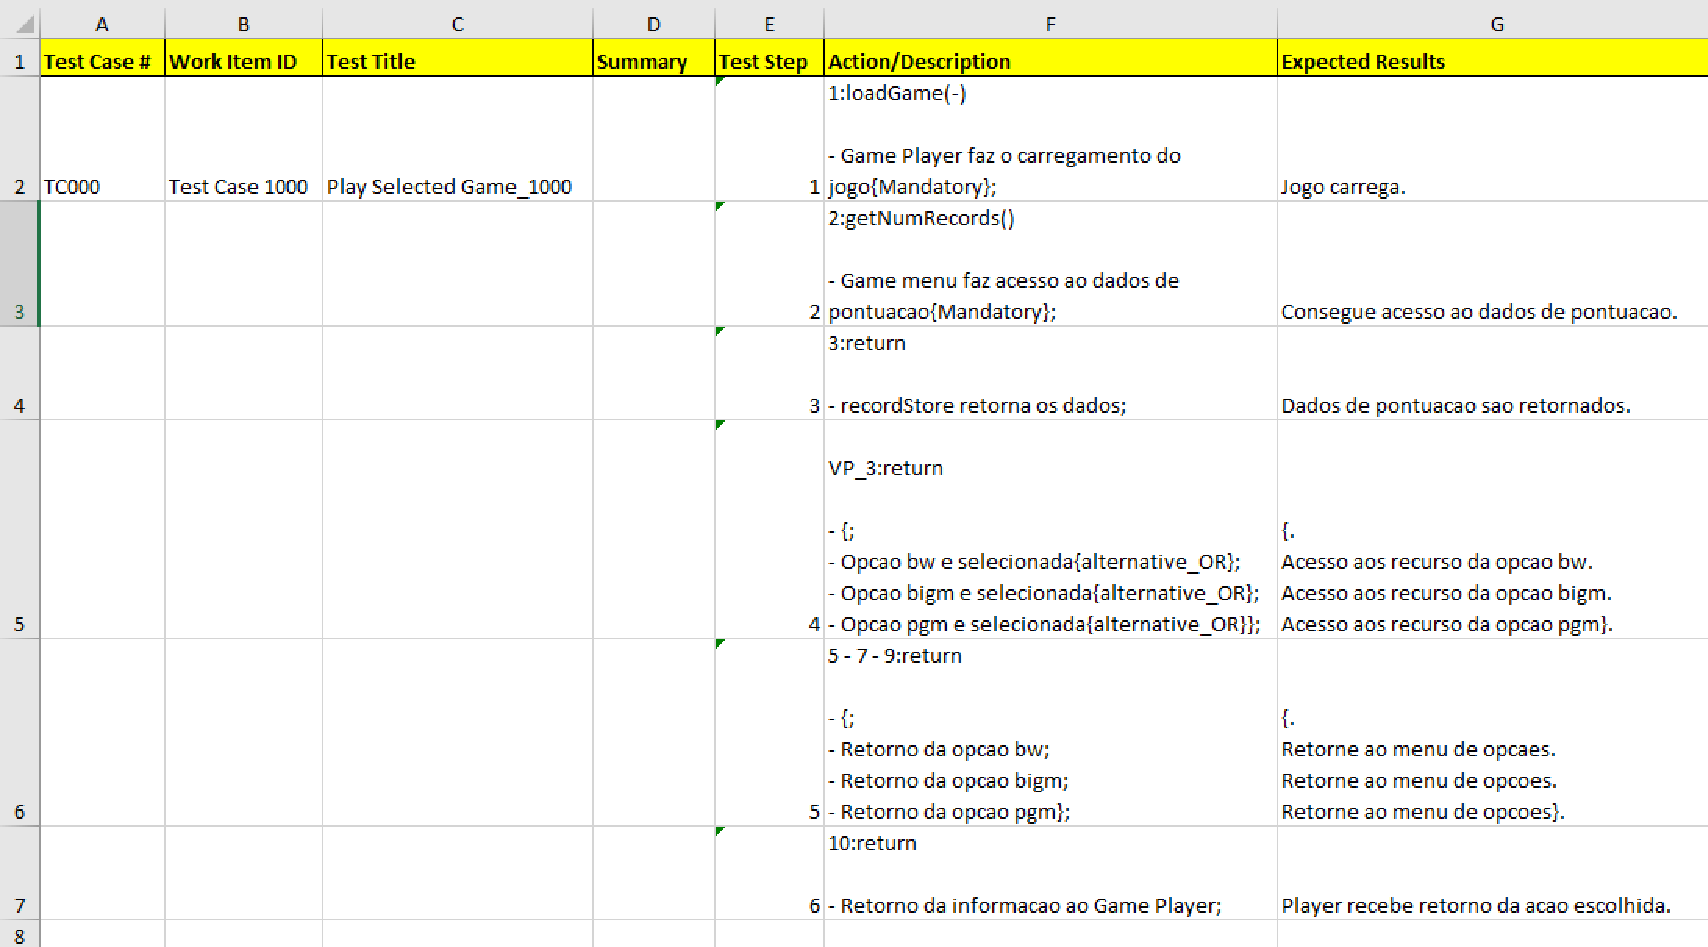
\includegraphics[scale=0.55]{splitcasodeteste.pdf}
	\caption{Arquivo XLSx com os casos de testes gerados}
	\label{fig:split_casodeteste}
\end{figure}
\newpage
\subsection{Resolução da Variabilidade}
\label{cap3subsec:solucao_variabilidade}

\textit{SMartyTesting} trata inicialmente a resolução da variabilidade no mesmo formato que SPLiT-MBt trata, onde as sequências de casos de teste são geradas contendo a variabilidade sem a resolução. Isso é importante quando se aborda a questão da reutilização, uma vez que quando novos produtos são gerados, a variabilidade pode sofrer alterações, ou haver mais pontos de variação. 

A viabilidade se torna desconhecida justamente por essa diferenciação que pode ser extensa, muitas instâncias e, quando se fala em reaproveitamento, a diferença pode sofrer um aumento e diferenciação, o que torna inviável a solução durante a modelagem.

Nesse caso, \textit{SMartyTesting} gera as sequências de teste com a variabilidade sem resolução, para que o engenheiro de software faça a tomada de decisão na engenharia de aplicação, analisando a melhor solução para a resolução da variabilidade contida.   


\subsection{Limitações de Uso da SPLiT-MBt}
\label{cap3subsec:limitacoes}

Por se estar utilizando ferramentas de apoio de terceiros, era previsto que limitações poderiam ser encontradas. Nesse caso, foram encontradas limitações em ambas as etapas.

Na primeira, com relação à utilização da notação \textit{SMarty} no mapeamento de conversão, pois \textit{Control Flow Analysis of UML 2.0 Sequence Diagrams} não cita soluções sobre variabilidade, embora, não sejam encontrados obstáculos sobre notações na utilização, a limitação ocorre somente por não ter uma regra explícita sobre notação de variabilidade.

Já na segunda etapa, envolvendo a aplicação de SPLiT-MBt, as limitações são mais significativas, embora não tenham influenciado nas validações. As limitações estão ligadas diretamente à estrutura do metamodelo do diagrama de atividades (\ref{fig:mapeamento2}).

SPLiT-MBt não fornece suporte a dois itens de \textit{ControlNode}, \textit{ForkNode} e \textit{JoinNode}, em testes com programação concorrente (atividades simultâneas). 

Outro ponto de limitação está ligado à continuidade de uma atividade após um \textit{DecisionNode} em que não são aceitas sub atividades a não ser que seja um estado de \textit{Merge}. Assim, considera-se isso uma não conformidade com sub-sistemas representados no artefato de entrada, um exemplo seria um \textit{InitialNode} vide (\ref{fig:mapeamento4}).  

Em um processo que não seja automatizado pode haver ameaças ao funcionamento, nesse caso a primeira etapa. Por esse motivo, é recomendado em trabalhos futuros a implementação e automatização de todos os processos do início ao fim do ciclo.

Pode-se considerar outra ameaça ao funcionamento da \textit{Control Flow Analysis of UML 2.0 Sequence Diagrams}, a metodologia de mapeamento. Por  não conter uma regra explícita sobre variabilidade, pode-se entender que a interpretação errada de uma das regras ocasione um erro de conversão. 


\section{Considerações Finais}
\label{cap3sec:consideracoes_smarty}
Neste tópico foi apresentada a estrutura de utilização da abordagem \textit{SMartyTesting}, partindo da caracterização da abordagem, a definição dos processos e o porquê das escolhas dos artefatos utilizados. Foi apresentado o modelo de conversão de DS para DA e as ferramentas utilizadas nas etapas posteriores. Na especificação detalhada, as duas etapas, em que se conta com o artefato de entrada DS, faz-se conversão para DA que é o artefato de entrada para a etapa seguinte. 